%!TEX TS-program = xelatex
\documentclass[../journal_main.tex]{subfiles}
\DeclareMathOperator*{\barr}{\scalerel*{+}{\textstyle\sum}}

\begin{document}
\chapter{Singlet constraint}
The $\mathbb{Z}_2$ gauge theory Hamiltonian is given by 
\begin{equation}
    H = - \sum_{p} J_p B_p - \sum_{l} h_e {X}_e
\end{equation}
where $B_p = \prod_{l \in p} {Z}_e$ with $p$ denoting a plaquette of spin links $e$ in the lattice. On a torus (periodic boundary) conditions, we get an additional constraint 
\begin{equation*}
    \prod_{p} {B}_p = \mathbb{I}
\end{equation*}
If we now perform a dual mapping of this theory by identifying the following
\[
    B_p = \sigma^x_p, \qquad X_e = \sigma^z_{p_e} \sigma^z_{p'_e}
\]
The dual Hamiltonian then becomes 
\begin{equation}
    H_\text{dual} = - \sum_p J_p \sigma^x_p - \sum_e h_e \sigma^z_{p_e} \sigma^z_{p'_e}
\end{equation}
which is the Transverse Field Ising Model (TFIM) Hamiltonian. However, now the constraint of periodic boundary conditions from $\mathbb{Z}_2$ gauge theory carries on forward to generate the following constraint on the TFIM
\[
    \prod_p B_p = \boxed{\prod_p \sigma^x_p = \mathbb{I}}
\]
The above is known as the \textbf{singlet constraint}.

\section{Quantum-to-Classical correspondance}
To perform Monte Carlo on the singlet-Ising model, 
\begin{equation}
    H = - \sum_p J_p \sigma^x_p - \sum_e h_e \sigma^z_{p_e} \sigma^z_{p'_e}\:\:, \qquad \prod_p \sigma^x_p = \mathbb{I}
    \label{Htfim}
\end{equation}  
we map the $d$-dimensional quantum Hamiltonian to a $d+1$-dimensional generalised classical Ising model using the path integral. In the end, we obtain the effective action with singlet constraint imposed
\begin{equation}
    S_s[\{\sigma\}] = -\sum_{l}\sum_{e} (\Delta \tau) h_e \sigma_{p_e}(l) \sigma_{p'_e}(l) - \sum_l \ln \cosh \qty[- \sum_p K_p \sigma_p(l+1) \sigma_p(l)] 
\end{equation}
where $\sigma$'s are now the classical spin variables $\in \{-1,1\}$, and the label $l$ denotes the summation over the imaginary time domain such that $l \in \{1, \ldots N_\tau\}$ and $\sigma_i(N_\tau +1) = \sigma_i(1)$ with $N_\tau \Delta \tau = \beta$. The newly defined $K_p$ is  
\[
    K_p = -\frac{1}{2} \ln \tanh\qty(\frac{\beta J_p}{N_\tau})  
\]
For a $1$-dimensional TFIM (with singlet constraint), the corresponding $2$-dimensional generalised Ising model comes out as
\begin{equation}
    S[\{\sigma\}] = -\sum_{l=1}^{N_\tau}\sum_{i=1}^{N_x} (\Delta \tau) h_i \sigma_{i}(l) \sigma_{i+1}(l) - \sum_{l=1}^{N_\tau} \ln \cosh \qty[- \sum_{i=1}^{N_x} K_i \sigma_i(l+1) \sigma_i(l)]
    \label{1Dtfimto2Dcim}
\end{equation}  

\section{Alignment observable}
Carefully analyzing the term $\sigma_i(l) \sigma_i(l+1)$ in Eqn. \eqref{1Dtfimto2Dcim}, we see that
\begin{itemize}
    \item $\sigma_i(l) \sigma_i(l+1) = -1$ if $\sigma_i(l) = - \sigma_i(l+1) \quad \implies$ \textbf{anti-aligned pair} ,
    \item $\sigma_i(l) \sigma_i(l+1) = +1$ if $\sigma_i(l) = + \sigma_i(l+1) \quad \implies$ \textbf{aligned pair}. 
\end{itemize}
Therefore, the term $\sum_i \sigma_i(l) \sigma_i(l+1)$ acts like a ``measure of alignment'' between spins in adjacent layers, contributing $+1$ to the sum if a pair is aligned, and $-1$ if the pair is anti-aligned. Hence, we define a new \textbf{alignment observable}  $A(l)$
\begin{equation}
    A(l) \equiv \frac{1}{N_x} \sum_{i=1}^{N_x} \sigma_i(l) \sigma_i(l+1) = \frac{1}{N_x}\qty(N_a(l) - N_o(l)) \quad \in [-1, 1] 
\end{equation}
where $N_a(l)$ is the number of aligned and $N_o(l)$ is the number of opposite (anti-aligned) spin pairs in adjacent layers $l$ and $l+1$. If we further keep the coupling strengths constant, our effective action becomes
\begin{equation}
    S = -h \Delta \tau  \sum_{i=1}^{N_x} \sum_{l=1}^{N_\tau} \sigma_i(l) \sigma_i(l+1) - \sum_{l=1}^{N_\tau} \ln \cosh \qty[-K N_x A(l)] .
    \label{effectiveaction}
\end{equation}
An interesting point to note is that the action is agnostic to the sign of the alignment $A(l)$, which implies that an ``alignment flip'' is a subsystem symmetry of Eqn. \eqref{effectiveaction}. 

\section{Subsystem symmetry breaking}
The effective action in Eqn. \eqref{effectiveaction} possesses the following subsystem symmetry 
\[
    \hat{F}(l) = \prod_{i \in \text{layer } l} \hat{X}_{(i,l)}
\]
i.e. flipping all the spins in layer $l$, or an \textbf{alignment flip} $A(l) \rightarrow -A(l)$,  leaves the $S$ invariant. Therefore, both $A(l) = +A$ and $A(l) = -A$ states should be equally probable. ~\\~\\
However, as we increase the system size $N_x \gg 1$, the minima of $S$ get deeper, and the system chooses either the $A(l) \approx +1$ or $A(l) \approx -1$ state and stays there, unable to cross the energy barrier to go to the other side of the configuration space.~\\~\\
Even though $S$ possesses the subsystem symmetry, these states don't. This is known as \textbf{subsystem symmetry breaking}, and $A(l)$ acts like an order parameter for this system (just like $m$ in 2D Ising model with $\mathbb{Z}_2$ symmetry breaking in the low temperature limit).

\section{Metropolis Monte Carlo algorithm}

To demonstrate the process of subsystem symmetry breaking in the model, we show how single spin-flips in Metropolis algorithm are unable to let the system cross the energy barrier and explore the other parts of the configuration space.~\\~\\
In our algorithm, we keep $\Delta \tau = 1$ fixed, $\implies \beta = N_\tau $. So the ground state of the model can be analysed by choosing a large enough $N_\tau $ to emulate $\beta \to \infty$ limit.~\\~\\
An algorithm for performing Metropolis on our model of interest is as follows
\begin{algorithm}{singlet-metropolis}
    \> define $\sigma[N_x ,N_\tau];$ \\
    \> \text{initialize spins (all up, hot-start, as input)} $\sigma[i, l]$;\\
    \> \text{define weighted alignment array} $\varepsilon[N_\tau];$ \\
    \> \text{initialize } $\varepsilon[l] = -\sum_i K_i \sigma_i(l+1) \sigma_i(l), \quad\forall\: l;$ \\
    \> \texttt{// Metropolis updates} \\
    \>{\bf for} $n \in \{1, 2, \ldots N_\text{samp}\}$ \\
    \>{\bf begin}\\
    \>\> \texttt{// Single Monte Carlo step} \\
    \>\>{\bf for} $m \in \{1, 2, \ldots N_x \cdot N_\tau \}$ \\
    \>\>{\bf begin}\\
    \>\>\> \text{choose site (random, sequential) }$:=(i_0, l_0)$;\\
    \>\>\> define $\varepsilon'_{l_0}, \:\:
    \varepsilon'_{l_0 - 1}; $\\
    \>\>\> define $\Delta S, \:\: \Delta S_x, \:\: \Delta S_t;$\\
    \\
    \>\>\> $\varepsilon'_{l_0-1} = \varepsilon[l_0-1] + 2K_{i_0}\cdot\sigma(i_0, l_0)\cdot\sigma(i_0, l_0-1);$\\
    \>\>\> $\varepsilon'_{l_0}\:\:\:\: = \varepsilon[l_0] \:\:\:\:\quad + 2K_{i_0}\cdot\sigma(i_0, l_0)\cdot\sigma(i_0, l_0+1);$\\
    \\
    \>\>\> $\Delta S_x = 2\Delta \tau \cdot h_{i_0} \cdot \sigma(i_0, l_0) \cdot [\sigma(i_0-1,l_0) + \sigma(i_0+1,l_0)];$ \\
    \>\>\> $\Delta S_t = \ln \qty[\cosh(\varepsilon[l_0])/\cosh(\varepsilon'_{l_0})] + \ln\qty[\cosh(\varepsilon[l_0-1])/\cosh(\varepsilon'_{l_0-1})] ;$ \\
    \>\>\> $\Delta S = \Delta S_x + \Delta S_t ;$ \\ 
    \\
    \>\>\> define $p = $ random number; \\
    \>\>\>{\bf if} $p < \exp(-\Delta S)$\\  
    \>\>\>{\bf begin}\\
    \>\>\>\> $\varepsilon[l_0 - 1] = \varepsilon'_{l_0-1}$; \\
    \>\>\>\> $\varepsilon[l_0] \:\:\:\:\quad =  \varepsilon'_{l_0}$; \\
    \>\>\>\> $\sigma[i_0, l_0] = (-1)\cdot \sigma[i_0, l_0];$\\
    \>\>\>{\bf end}\\
    \>\>{\bf end}\\
    \>{\bf end}\\
\end{algorithm}

\section{Metropolis simulation results}
\subsection{Expectation values of alignment}
To show that the subsystem symmetry is indeed broken for large spatial lattice sizes $N_x \gg 1$, we compute expectation value $\expval{A(l)}$, where $l$ labels the layers $\in \{1, 2, \ldots N_\tau\}$. ~\\~\\
For small spatial lattice sizes, we expect $\expval{A(l)} \approx 0$ since the energy barrier to jump between different parts of the configuration space isn't high enough. However, for larger spatial lattic sizes, we expect the action minima to get deeper, leading to the system state getting stuck in either of the $\expval{A(l)} \approx \pm 1$ states and unable to cross to the other side.~\\~\\
For the simulations, we use the following parameters
\begin{itemize}[label={}]
    \setlength{\itemsep}{0.1em}
    \item \texttt{spatial lattice size } $N_x \in \{ \texttt{2, 3, 4 $\ldots$, 20} \}$  
    \item \texttt{no of sampling sweeps } $N_\text{samp} \in \{\texttt{2.0e4, 6.0e4, 1.0e5, $\ldots$, 2.6e5, 3.0e5} \}$
    \item \texttt{imaginary time lattice size } $N_\tau = $ \texttt{40}, \: $\Delta \tau = $ \texttt{1.0}
    \item \texttt{coupling constants} $K, h = $ \texttt{1.0} 
\end{itemize}

%%% FIG %%%
\begin{figure}[!htb]
    \centering
    \begin{subfigure}[b]{0.47\textwidth}
        \centering
        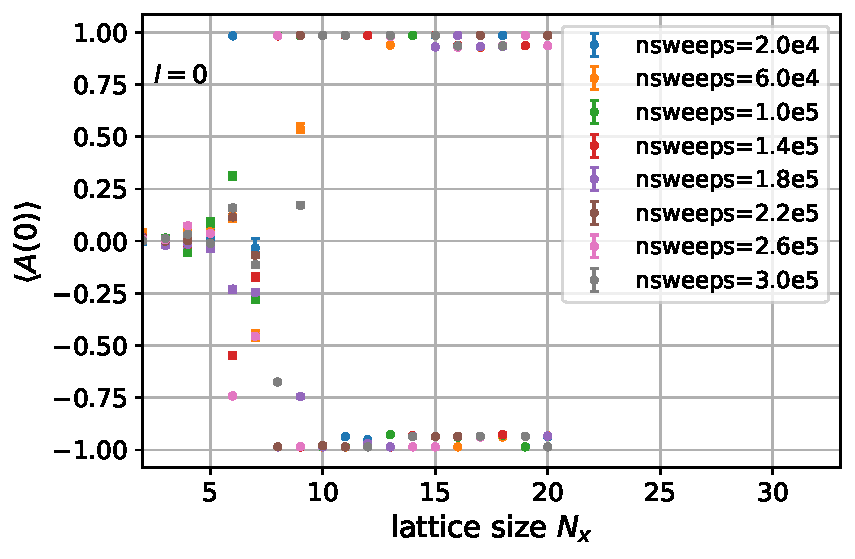
\includegraphics[width=\textwidth]{images/expval(A_l)_vs_N_x/A vs N_x (l=0).pdf}
        \caption{$\expval{A(0)} \text{ vs } N_x$}
    \end{subfigure}
    \hspace{1em}  %\hfill
    \begin{subfigure}[b]{0.47\textwidth}
        \centering
        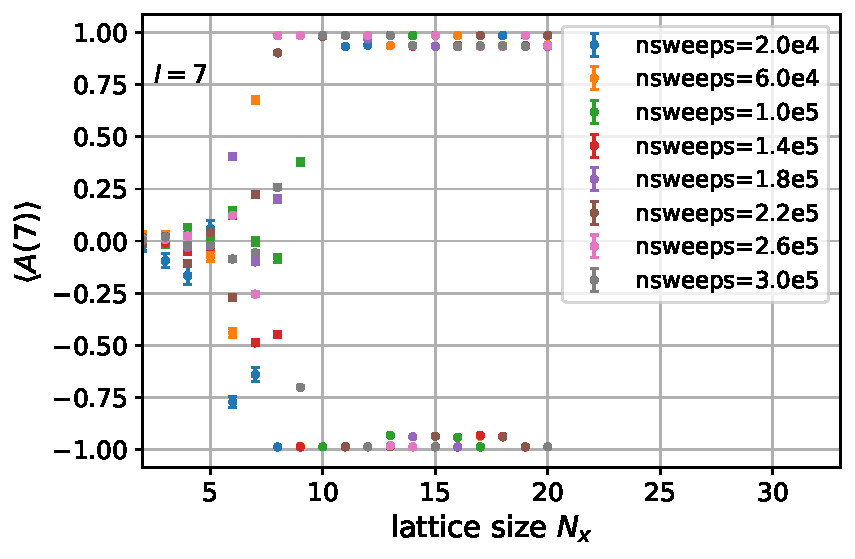
\includegraphics[width=\textwidth]{images/expval(A_l)_vs_N_x/A vs N_x (l=7).pdf}
        \caption{$\expval{A(7)} \text{ vs } N_x$}
    \end{subfigure}
    \caption{$\expval{A(l)}$ for different values of $l$ calculated for different number of Monte Carlo sweeps.}
    \label{expvalA(l)_vs_N_x}
\end{figure}
%%% FIG %%%

%%% FIG %%%
\begin{figure}[!htb]\ContinuedFloat
    \centering
    \begin{subfigure}[b]{0.47\textwidth}  %keep total sum <1 to show in same line
        \centering
        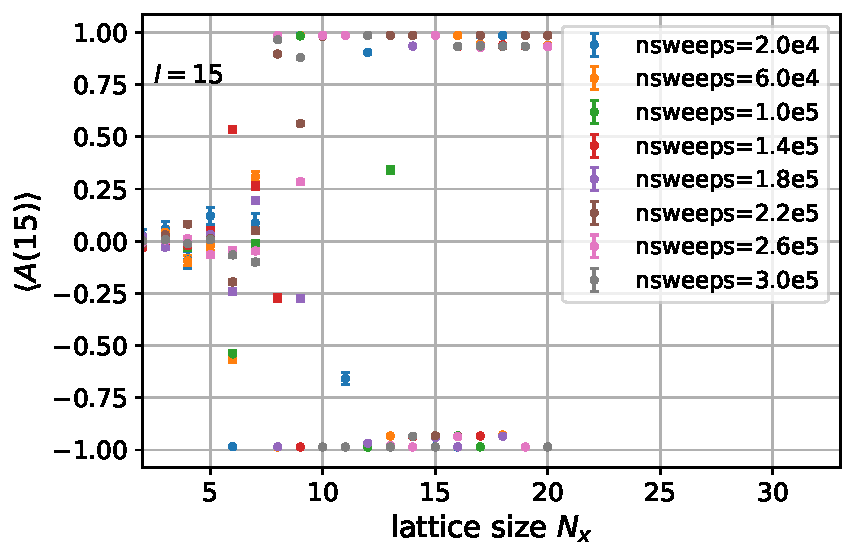
\includegraphics[width=\textwidth]{images/expval(A_l)_vs_N_x/A vs N_x (l=15).pdf}
        \caption{$\expval{A(15)} \text{ vs } N_x$}
    \end{subfigure}
    \hspace{1em}  %\hfill
    \vspace{1em}
    \begin{subfigure}[b]{0.47\textwidth}
        \centering
        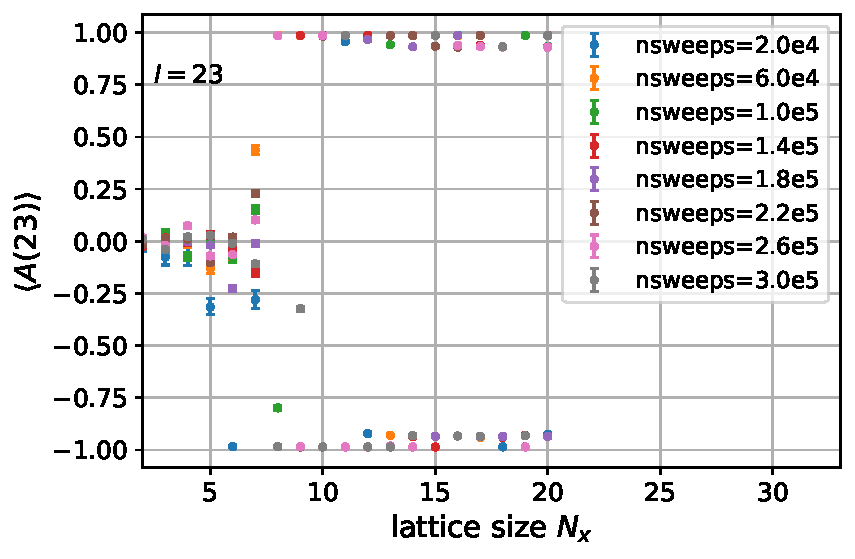
\includegraphics[width=\textwidth]{images/expval(A_l)_vs_N_x/A vs N_x (l=23).pdf}
        \caption{$\expval{A(23)} \text{ vs } N_x$}
    \end{subfigure}
    \hspace{1em}  %\hfill
    \vspace{1em}
    \begin{subfigure}[b]{0.47\textwidth}
        \centering
        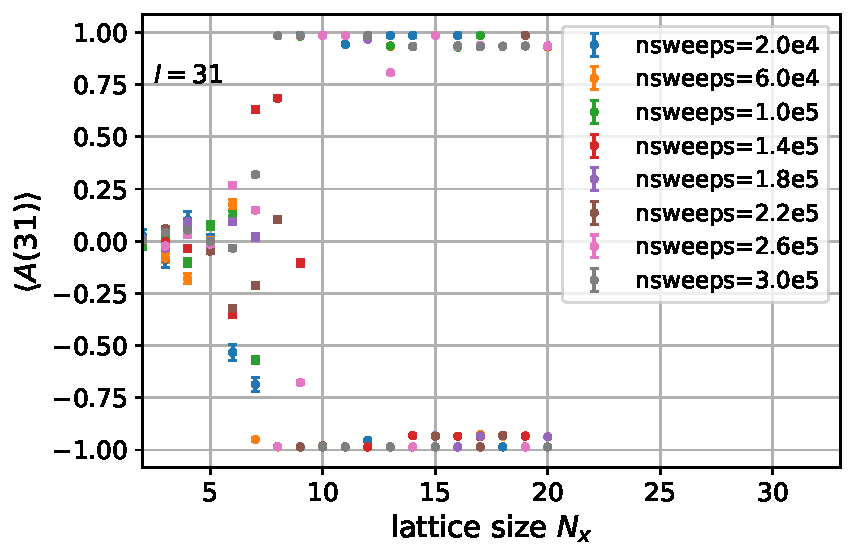
\includegraphics[width=\textwidth]{images/expval(A_l)_vs_N_x/A vs N_x (l=31).pdf}
        \caption{$\expval{A(31)} \text{ vs } N_x$}
    \end{subfigure}
    \hspace{1em}  %\hfill
    \begin{subfigure}[b]{0.47\textwidth}
        \centering
        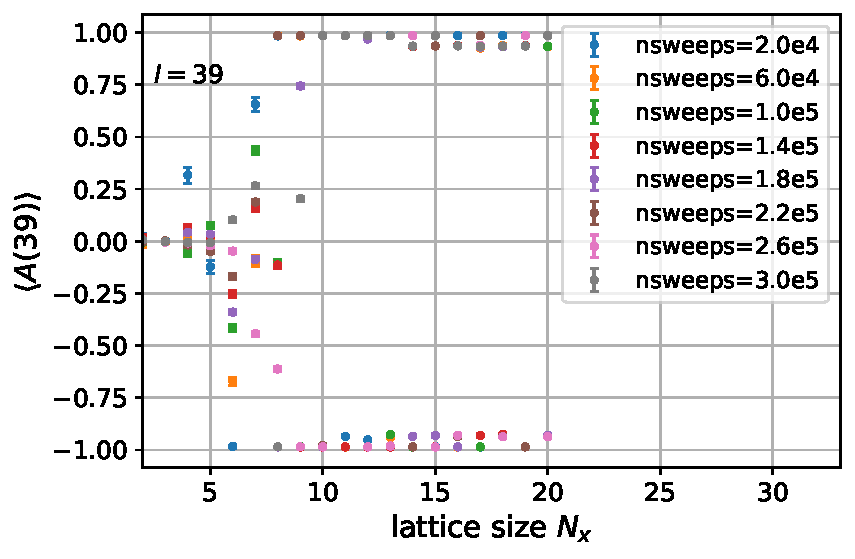
\includegraphics[width=\textwidth]{images/expval(A_l)_vs_N_x/A vs N_x (l=39).pdf}
        \caption{$\expval{A(39)} \text{ vs } N_x$}
    \end{subfigure}
    \caption{$\expval{A(l)}$ for different values of $l$ calculated for different number of Monte Carlo sweeps.}
\end{figure}
\FloatBarrier
As can be seen from Fig. \ref{expvalA(l)_vs_N_x}, the plots for $\expval{A(l)}$ vs $N_x$ look roughly the same, suggesting that the expectation values themselves are independent of the chosen layer. This can also be seen in Fig. \ref{differentlayer_sameMCsweeps} where we have plotted $\expval{A(l)}$ vs $N_x$ for two different layers (for the same number of Monte Carlo sweeps). With the same number of MC sweeps to explore the configuration space, we see that the plots for both the layers $l_1$ and $l_2$ fall into the broken symmetry state around the same value of $N_x \approx 8$. This demonstrates that all the layers $l$ show roughly the same dynamics, i.e. in the high spatial lattice size limit $N_x \gg 1$, they get stuck in either of the $\expval{A(l)} \approx \pm 1$ wells, and aren't able to escape it, resulting in a bifurcation-like envelope stucture.~\\~\\
Another interesting point to note from Fig. \ref{expvalA(l)_vs_N_x} is the dependence of $\expval{A(l)}$ on the number of Monte Carlo sweeps \texttt{nsweeps}. As we increase \texttt{nsweeps}, we see that it takes a relatively higher spatial lattice size $N_x$ to obtain $\expval{A(l)} \not\approx 0$ i.e. the bifurcation to non-zero $\expval{A(l)}$ is delayed. This is because as we increase \texttt{nsweeps}, the Monte Carlo run gets the opportunity to explore a larger part of the configuration space, and the probability to explore the other side of the configuration space increases, hence resulting in $\expval{A(l)} \approx 0$ for relatively larger $N_x$. However, beyond a certain $N_x$, the Metropolis acceptance probability is too low to explore configuration space even with very large \texttt{nsweeps}.       
%%% FIG %%%
\begin{figure}[!htb]
    \centering
    \begin{subfigure}[b]{0.57\textwidth}
        \centering
        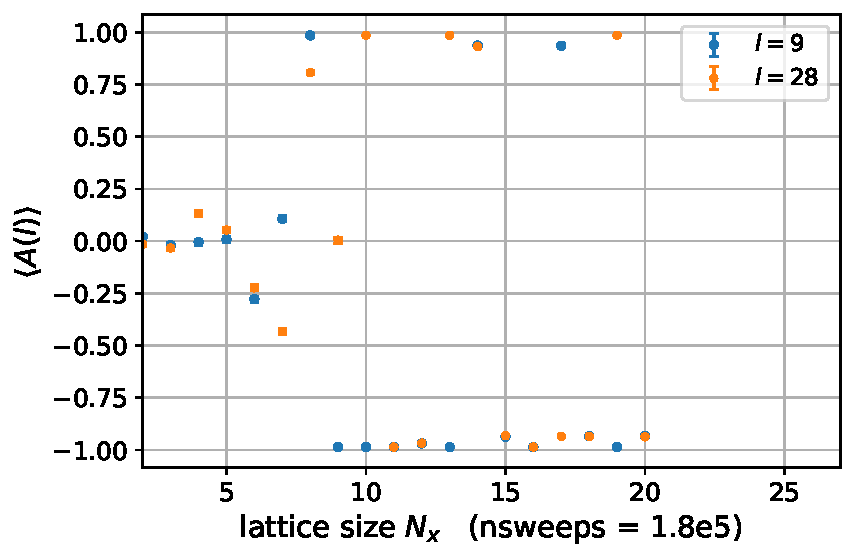
\includegraphics[width=\textwidth]{images/expval(A_l)_vs_N_x/A vs N_x (nsweeps=1.8e5).pdf}
    \end{subfigure}
    \caption{$\expval{A(l)}$ vs $N_x$ for two different layers $l_1 = 9,\: l_2 = 28$ ran over \texttt{nsweeps = 1.8e5}.}
    \label{differentlayer_sameMCsweeps}
\end{figure}
%%% FIG %%%
\FloatBarrier
\subsection{Autocorrelation Times of alignment}
Another way to demonstrate the expected subsystem symmetry breaking of this system is to look at autocorrelation times of $\expval{A(l)}$. Since we expect the system to get stuck in either of the $A(l) \approx \pm 1$ minima, the temporal evolution of $A(l)$ should be highly autocorrelated.~\\~\\
For the ease of writing, we will briefly switch to writing $A(l)$ as $A_l$. So, for the observable $A_l$, the autocorrelations are computed as 
\begin{equation}
    \text{Autocorr}[A_l] = \frac{\expval{A_l(k) A_l(k+T)}}{\expval{A_l(k)^2}} = \frac{1}{N-T} \sum_{k=0}^{N-T-1} \frac{A_l(k) \cdot A_l(k+T)}{\expval{A_l(k)^2}}
\end{equation} 
where the average is taken over the first $N-T$ measurements, i.e.
\[
    \expval{A_l(k)^2} = \frac{1}{N-T} \sum_{k=0}^{N-T-1} [A(k)]^2
\] 
One might notice that this definition of autocorrelation function looks a bit different, as it is computing the sum over the measurements themselves, and not over their deviations i.e. $\expval{A_l(k) A_l(k+T)} - \expval{A_l(k)}^2$. This is because we have forced $\expval{A_l} = 0$, since that is the general expectation due to the subsystem symmetry. If we don't force $\expval{A_l} = 0$, we would calculate autocorrelations for the system oscillating in one of the minima wells, which isn't what we desire.~\\~\\
In the following simulation, we have \texttt{nsweeps = 2.0e4}, $N_x = $ \texttt{20}, $N_\tau = $ \texttt{40}, $\Delta \tau = $ \texttt{1.0}, and the autocorrelations are computed for $T \in \{ $ \texttt{1, 2, $\ldots$, 3000} $\}$.       

%%% FIG %%%
\begin{figure}[!htb]
    \centering
    \begin{subfigure}[b]{0.5\textwidth}
        \centering
        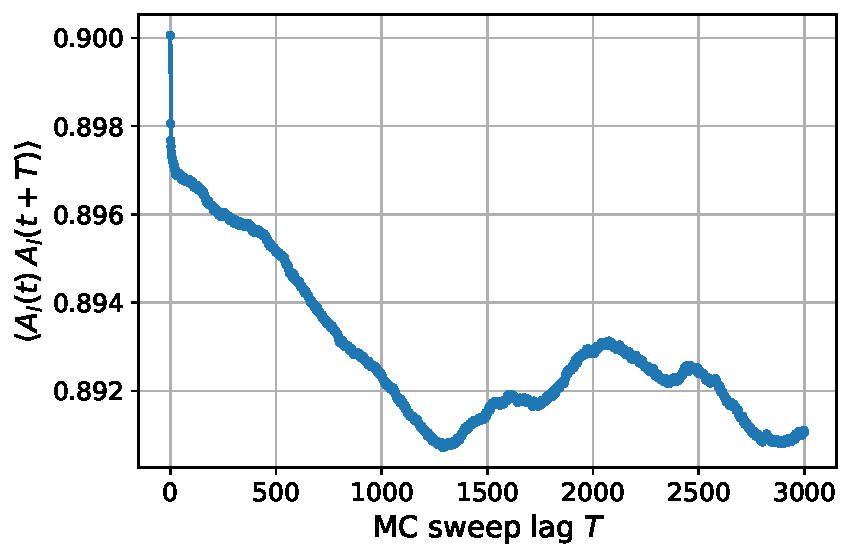
\includegraphics[width=\textwidth]{images/misc/autocorrfn_singlet.pdf}
    \end{subfigure}
    \caption{Autocorrelation function $\expval{A_l(k) A_l(k+T)}$.}
    \label{autocorrs_singlet}
\end{figure}
%%% FIG %%%
\FloatBarrier

As can be seen in Fig. \ref{autocorrs_singlet}, the autocorrelation function stays nearly constant $\approx 0.89$ even for $T = 3000$, which implies that autocorrelation time $\boxed{\tau \to \infty}$ for $A(l)$. Hence, once the system gets stuck in one of the minimas, it almost never gets the chance to escape it just by using single spin-flips. 

\section{Fixing the subsystem symmetry}
To ensure that our subsystem symmetry remains unbroken (or alternatively, to stay in the singlet sector of the Hilbert space), we need the classical system to explore the configuration space equally on both sides of $A(l)$. A possible resolution is to perform ${f N_x}$  \textbf{random spin flip proposals} followed by a \textbf{random alignment flip}, where $f \in \mathbb{R}^+$ with $f \to \infty$ limit implying no alignment flips.\\~\\~
The above combination in theory still equilibriates to the Boltzmann distribution because an alignment flip is a $\Delta S = 0$ change, i.e. it is a proposal which is \textbf{always accepted} in Metropolis MCMC. This new prescription defines a single Monte Carlo sweep as a combination of $N_x N_\tau$ spin flip proposals and $\left\lfloor N_\tau/f \right\rfloor$ alignment flips. We expect alignment flips with $f \sim \mathcal{O}(1)$ to restore the subsystem symmetry in our classical system.

\subsection{Simulation results with alignment flips}
We use the following parameters for the simulation :
\begin{itemize}[label={}]
    \setlength{\itemsep}{0.1em}
    \item \texttt{alignment flip fraction $f = $ 2.0}
    \item \texttt{spatial lattice size } $N_x \in \{ \texttt{2, 4, 6 $\ldots$, 32} \}$  
    \item \texttt{no of sampling sweeps $N_\text{samp} = $ 5.0e4} 
    \item \texttt{imaginary time lattice size } $N_\tau = $ \texttt{40}, \: $\Delta \tau = $ \texttt{1.0}
    \item \texttt{coupling constants} $K, h = $ \texttt{1.0} 
\end{itemize}
We perform the simulations both with and without alignment flips, and compare the expectation value of the alignment observable $A(l)$. 
%%% FIG %%%
\begin{figure}[!htb]
    \centering
    \begin{subfigure}[b]{0.57\textwidth}
        \centering
        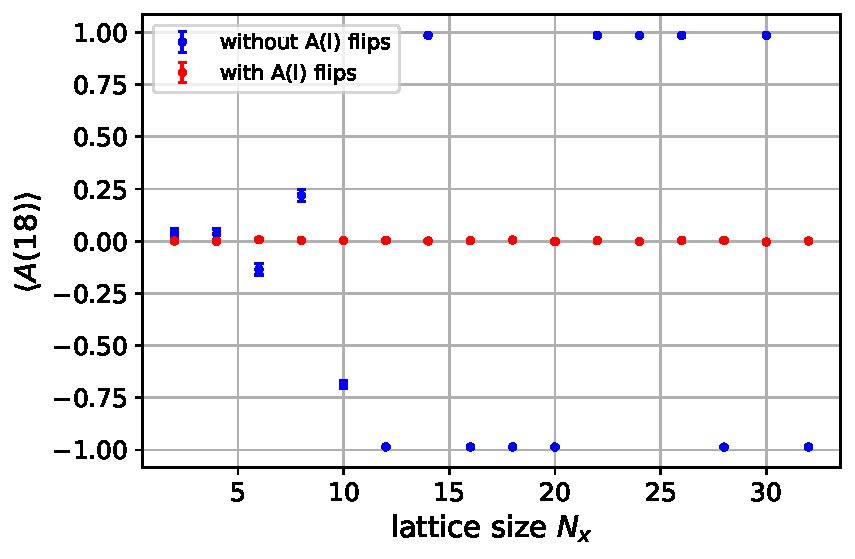
\includegraphics[width=\textwidth]{images/fix_subsystem_symmetry/expval(A(l)) vs N_x (l=18) with and without aflips.pdf}
    \end{subfigure}
    \caption{$\expval{A(l = 18)}$ both with and without alignment flips for different spatial lattice sizes.}
    \label{alignflipexpval}
\end{figure}
%%% FIG %%%
\FloatBarrier
As expected, the alignment flips make the configuration space equally accessible towards both the $A(l)\approx \pm 1$ sides resulting in $\expval{A(l)} \approx 0$ as shown in Fig. \ref{alignflipexpval}. This is further confirmed if one plots the $A(l)$ measurements as a function of Monte Carlo sweeps for a given layer $l$ when we introduce alignment flips.  
 
%%% FIG %%%
\begin{figure}[!htb]
    \centering
    \begin{subfigure}[b]{0.47\textwidth}
        \centering
        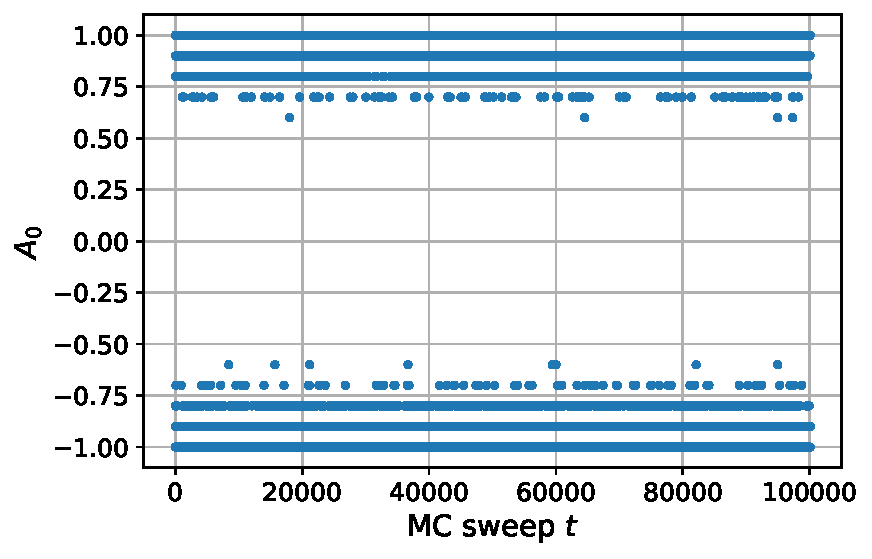
\includegraphics[width=\textwidth]{images/fix_subsystem_symmetry/measurement A(l) vs MC time (l=0).pdf}
        \caption{ $A(l)$ measurements vs MC time.}
    \end{subfigure}
    \hspace{1em}  %\hfill
    \begin{subfigure}[b]{0.45\textwidth}
        \centering
        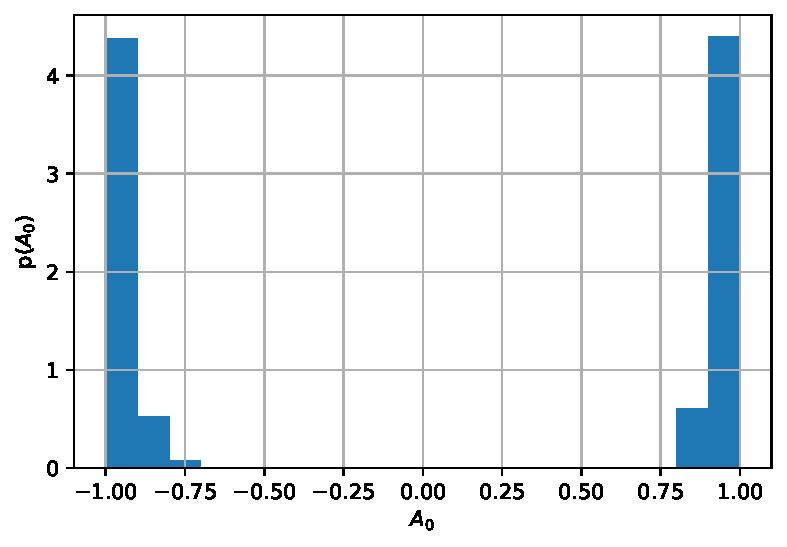
\includegraphics[width=\textwidth]{images/fix_subsystem_symmetry/measurement A(l) histogram (l=0).pdf}
        \caption{ $A(l)$ measurements histogram.}
    \end{subfigure}
    \caption{Configuration space exploring both $A(l)>0$ and $A(l)<0$ sectors \textbf{with} alignment flips.}
    \label{alignflipmeasurements}
\end{figure}
%%% FIG %%%
\FloatBarrier

Fig. \ref{alignflipmeasurements} clearly shows that introducing alignment flips makes the configuration space traverse both the $A(l)>0$ and $A(l)<0$ sectors of the state space, hence ensuring that the ergodicity and consequently the subsystem symmetry of the classical system is preserved.   

\subsection{Autocorrelation times}
Since we were successfully able to explore both the sides of the configuration space using alignment flips, we consequently expect the autocorrelation times to also go down substantially since the system is no longer stuck.~\\~\\
Since the system isn't stuck in a minima well now, we can now use the usual definition for the autocorrelation function 
\begin{equation}
    \text{Autocorr}[A_l] = \frac{1}{N-T} \sum_{k=0}^{N-T-1} \frac{(A_l(k) - \expval{A_l}) \cdot (A_l(k+T) - \expval{A_l}}{\expval{A_l(k)^2}}
\end{equation} 
where the average is taken over the first $N-T$ measurements, i.e.
\[
    \expval{A_l(k)^2} = \frac{1}{N-T} \sum_{k=0}^{N-T-1} [A(k)]^2
\] 
%%% FIG %%%
\begin{figure}[!htb]
    \centering
    \begin{subfigure}[b]{0.5\textwidth}
        \centering
        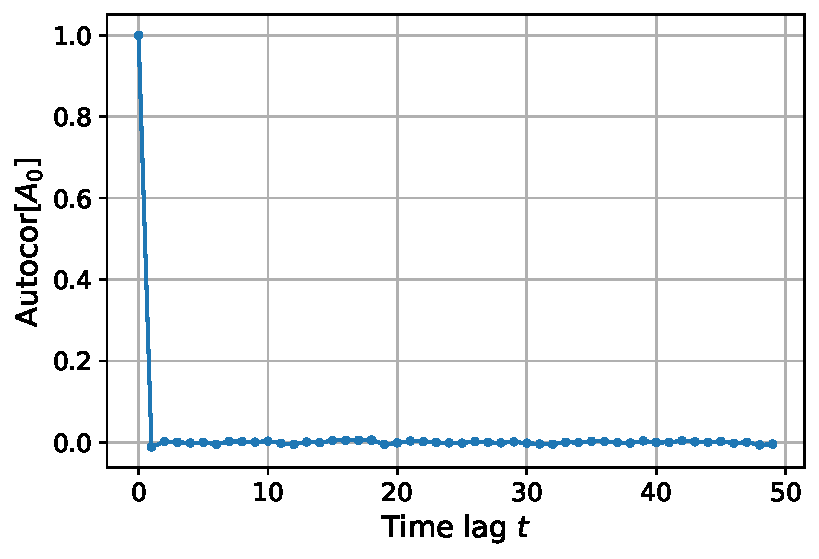
\includegraphics[width=\textwidth]{images/fix_subsystem_symmetry/Autocor[A(l)] (l=0).pdf}
    \end{subfigure}
    \caption{Autocorrelation function \textbf{with} alignment flips.}
    \label{alignflipautocorr}
\end{figure}
%%% FIG %%%
\FloatBarrier
As is apparent from Fig. \ref{alignflipautocorr}, the autocorrelations drop extremely quickly, and for this particular simulation we obtained $\boxed{\tau_\text{int} = 0.529}$ implying that the alignment measurements $A(l)$ are highly uncorrelated in the Monte Carlo simulation.   

\section{Mapping quantum operators to classical observables}
So far, we have been able to conclude that performing Metropolis MCMC as a combination of spin flips and alignment flips keeps the subsystem symmetry of our system intact, and can be a reliable way to perform calculations on using the Quantum to Classical correspondance duality.~\\~\\ 
However, the only way to cross-check our results is to calculate the expectation value of an operator $\hat{\mathcal{O}}$ in the system described by $\hat{H}_\text{TFIM}$ \eqref{Htfim} in the singlet basis using an Exact Diagonalization approach, and compare it to the expectation value of the corresponding classical observable $\mathcal{O}_\text{classical}$ using Metropolis MCMC. In this subsection, we'll describe a method of mapping the quantum operators to the corresponding classical observables.~\\~\\
\subsection{Types of operators in consideration}
To begin with, any operator $\hat{\mathcal{O}}$ defined on the singlet sector Hilbert space must satisfy 
\begin{equation}
    \hat{S} \hat{\mathcal{O}} \hat{S} = \hat{\mathcal{O}}
    \label{operator}
\end{equation}
where $\hat{S} = \prod_i \hat{X}_i$ is the global flip operator. This is because the singlet constraint $\hat{S} = \mathbb{I}$ must be satisfied on $\mathcal{H}_s$. This can also be seen by the following argument - any operator $\mathcal{O}$ defined on $\mathcal{H}_s$ can be written in the outer product notation as 
\[
    \hat{\mathcal{O}} = \sum_{i,j} c_{ij} \hat{P}\ket{\{\sigma\}}_i \bra{\{\sigma '\}}_j \hat{P}
\]     
where $\hat{P} = (\mathbb{I} + \hat{S})/2$, so the sandwich between $\hat{S}$'s will give 
\begin{equation*}
    \hat{S} \hat{\mathcal{O}} \hat{S} = \sum_{ij} c_{ij} \underbrace{\hat{S}\hat{P}}_{ = \hat{P}} \ket{\{\sigma\}}_i \bra{\{\sigma '\}}_j \underbrace{\hat{P} \hat{S}}_{ = \hat{P}} = \sum_{i,j} c_{ij} \hat{P}\ket{\{\sigma\}}_i \bra{\{\sigma '\}}_j \hat{P} = \hat{\mathcal{O}}
\end{equation*}
Therefore, any operator on the singlet sector $\mathcal{O}: \mathcal{H}_s \to \mathcal{H}_s$ must satisfy  \eqref{operator}.~\\~\\
Some elementary operators which satisfy the above constraint are 
\begin{itemize}
    \setlength{\itemsep}{0.1em}
    \item $\hat{Z}_i \hat{Z}_j$
    \item $\hat{X}_i$   
\end{itemize} 
We can now try mapping such relevant quantum operators to their corresponding classical analogues.  
We first note that the Hamiltonian is given by the form 
\[
    \hat{H} = - h \sum_i \hat{Z}_i \hat{Z}_j - J \sum_i \hat{X}_i 
\]
As always, the quantum expectation value of an operator is given by 
\begin{align*}
    \langle {\hat{\mathcal{O}}} \rangle  &= \frac{\Tr(e^{-\beta \hat{H}}\hat{\mathcal{O}})}{\Tr(e^{-\beta \hat{H}})} \\
    &= \frac{1}{\mathcal{Z}} \sum_{\{\sigma_0 \}} \sum_{\mu_0, \lambda_0 \in \{\pm 1\}} \mel{\{\mu_0 \sigma _0\}}{e^{-\Delta \tau \hat{H}} e^{-\Delta \tau \hat{H}} \ldots e^{-\Delta \tau \hat{H}} \hat{\mathcal{O}}}{\{\lambda_0 \sigma _0\}}    
\end{align*}
Using cyclicity of trace, we can say that $\hat{\mathcal{O}}$ does not have to be in the special position at the end of the operator product, therefore
\begin{align*}
    \mathcal{Z} \langle {\hat{\mathcal{O}}} \rangle & = \sum_{\{\sigma_0 \}, \mu_0, \lambda_0} \mel{\{\mu_0 \sigma _0\}}{e^{-\Delta \tau \hat{H}} e^{-\Delta \tau \hat{H}} \ldots e^{-\Delta \tau \hat{H}} \hat{\mathcal{O}}}{\{\lambda_0 \sigma _0\}} \\
    & + \sum_{\{\sigma_0 \}, \mu_0, \lambda_0} \mel{\{\mu_0 \sigma _0\}}{e^{-\Delta \tau \hat{H}} e^{-\Delta \tau \hat{H}} \ldots \hat{\mathcal{O}} e^{-\Delta \tau \hat{H}} }{\{\lambda_0 \sigma _0\}} \\
    & + \sum_{\{\sigma_0 \}, \mu_0, \lambda_0} \mel{\{\mu_0 \sigma _0\}}{e^{-\Delta \tau \hat{H}} \ldots \hat{\mathcal{O}} e^{-\Delta \tau \hat{H}} e^{-\Delta \tau \hat{H}} }{\{\lambda_0 \sigma _0\}} \\
    & \ldots  \: + \: \sum_{\{\sigma_0 \}, \mu_0, \lambda_0} \mel{\{\mu_0 \sigma _0\}}{\hat{\mathcal{O}} e^{-\Delta \tau \hat{H}} e^{-\Delta \tau \hat{H}} \ldots e^{-\Delta \tau \hat{H}}}{\{\lambda_0 \sigma _0\}}
\end{align*}
Defining $\mu_{N_\tau} = \mu_0, \lambda _{N_\tau} = \lambda _0$, and $\{\sigma_{N_\tau}\} = \{\sigma_0\}$, and inserting the singlet identity 
\[
    \mathbb{I}_s = \sum_{\{\sigma_l \}, \mu_l, \lambda_l} \ket{\{\lambda_{l} \sigma_{l}\}}\bra{\{\mu_{l} \sigma_{l}\}}
\] 
for $l \in \{1, 2, 3 \ldots, N_\tau - 1\}$, we get the following expression 
\begin{align}
    \mathcal{Z} \langle \hat{\mathcal{O}} \rangle = \qty(\prod_{l=0}^{N_\tau - 1} \sum_{\{\sigma_l \}, \mu_l, \lambda_l}) \frac{1}{N_\tau} \sum_{l_0 = 0}^{N_\tau - 1} \qty[\mel{\{\mu_{l_0+1} \sigma _{l_0+1}\}}{e^{-\Delta \tau \hat{H}} \hat{\mathcal{O}}}{\{\lambda_{l_0} \sigma _{l_0}\}} \cdot \prod_{l \neq l_0} \mel{\{\mu_{l+1} \sigma _{l+1}\}}{e^{-\Delta \tau \hat{H}}}{\{\lambda_{l} \sigma _{l}\}} ] 
    \label{generalop}
\end{align} 

\subsection{Classical analogue of $\hat{Z}_i \hat{Z}_j$}
We can now find the classical analogue of the $ \hat{\mathcal{O}} =  \hat{Z}_i \hat{Z}_j$ by performing the substitution in Eqn. \eqref{generalop}
\begin{align*}
    & \mathcal{Z} \langle {\hat{Z}_i \hat{Z}_j} \rangle \\
    & = \qty(\prod_{l=0}^{N_\tau - 1} \sum_{\{\sigma_l \}, \mu_l, \lambda_l}) \frac{1}{N_\tau} \sum_{l_0 = 0}^{N_\tau - 1} \qty[\mel{\{\mu_{l_0+1} \sigma _{l_0+1}\}}{e^{-\Delta \tau \hat{H}} {\hat{Z}_i \hat{Z}_j}}{\{\lambda_{l_0} \sigma _{l_0}\}} \cdot \prod_{l \neq l_0} \mel{\{\mu_{l+1} \sigma _{l+1}\}}{e^{-\Delta \tau \hat{H}}}{\{\lambda_{l} \sigma _{l}\}} ] \\
    & =  \qty(\prod_{l=0}^{N_\tau - 1} \sum_{\{\sigma_l \}, \mu_l, \lambda_l}) \frac{1}{N_\tau} \sum_{l_0 = 0}^{N_\tau - 1} \Bigg[\mel{\{\mu_{l_0+1} \sigma _{l_0+1}\}}{e^{-\Delta \tau \hat{H}}}{\{\lambda_{l_0} \sigma _{l_0}\}} (\lambda_{l_0} \sigma^i_{l_0})(\lambda_{l_0} \sigma^j_{l_0}) \\ 
    & \qquad \qquad \qquad \qquad \qquad \qquad \qquad \qquad \qquad \qquad \qquad \qquad \prod_{l \neq l_0} \mel{\{\mu_{l+1} \sigma _{l+1}\}}{e^{-\Delta \tau \hat{H}}}{\{\lambda_{l} \sigma _{l}\}}\Bigg] \\
    & = \qty(\prod_{l=0}^{N_\tau - 1} \sum_{\{\sigma_l \}, \mu_l, \lambda_l}) \qty(\frac{1}{N_\tau} \sum_{l_0 = 0}^{N_\tau - 1} \sigma^i_{l_0} \sigma^j_{l_0}) \qty[\prod_{l = 0}^{N_\tau - 1} \mel{\{\mu_{l+1} \sigma _{l+1}\}}{e^{-\Delta \tau \hat{H}}}{\{\lambda_{l} \sigma _{l}\}} ]
\end{align*} 
After manipulations on the $\prod_l$ product of terms, and performing a sum $\sum_{\mu_l, \lambda_l \in \{\pm 1\}}$, we get the usual partition function with the classical basis states 
\[
    \langle {\hat{Z}_i \hat{Z}_j} \rangle = \frac{1}{\mathcal{Z}} \qty(\prod_{l=0}^{N_\tau - 1} \sum_{\{\sigma_l \}}) \qty(\frac{1}{N_\tau} \sum_{l_0 = 0}^{N_\tau - 1} \sigma^i_{l_0} \sigma^j_{l_0}) e^{-S_\text{eff}}
\]   
where $S_\text{eff} = -h \Delta \tau \sum_{i}\sum_{l} \sigma^i_l \sigma^{i+1}_l - \sum_l \ln\cosh(K \sum_i \sigma^i_l \sigma^i_{l+1})$. Therefore, the classical observable corresponding to quantum operator $\hat{Z}_i \hat{Z}_j$ is 
\begin{equation}
    \boxed{
        O_{Z_i Z_j} = \frac{1}{N_\tau} \sum_{l = 0}^{N_\tau - 1} \sigma^i_{l} \sigma^j_{l}
    }
    \label{classicalzizj}
\end{equation}  

\subsection{Classical analogue of $\hat{X}_i$}
Following a similar procedure as above, we also calculate the classical observable corresponding to $\hat{X}_i$, although the calculation isn't as straightforward here 
\begin{align}
    & \mathcal{Z} \langle {\hat{X}_i} \rangle \nonumber \\
    & = \qty(\prod_{l=0}^{N_\tau - 1} \sum_{\{\sigma_l \}, \mu_l, \lambda_l}) \frac{1}{N_\tau} \sum_{l_0 = 0}^{N_\tau - 1} \qty[\mel{\{\mu_{l_0+1} \sigma _{l_0+1}\}}{e^{-\Delta \tau \hat{H}} \hat{X}_i}{\{\lambda_{l_0} \sigma _{l_0}\}} \cdot \prod_{l \neq l_0} \mel{\{\mu_{l+1} \sigma _{l+1}\}}{e^{-\Delta \tau \hat{H}}}{\{\lambda_{l} \sigma _{l}\}} ] \\
    \label{operator_x_i}
\end{align}
Let's first analyze the matrix element with $\hat{X}_i$
\[
    \mel{\{\mu_{l_0+1} \sigma _{l_0+1}\}}{e^{-\Delta \tau \hat{H}} \hat{X}_i}{\{\lambda_{l_0} \sigma _{l_0}\}} \approx \mel{\{\mu_{l_0+1} \sigma _{l_0+1}\}}{e^{-\Delta \tau \hat{H}_I} e^{-\Delta \tau \hat{H}_T} \hat{X}_i}{\{\lambda_{l_0} \sigma _{l_0}\}}
\] 
The above approximation is valid in the limit $\Delta \tau \to 0$ and $N_\tau \to \infty$. If we make the Ising interaction term $\hat{H}_I$ act on the bra at the left, we get
\begin{flalign*}
    & = \mel{\{\mu_{l_0+1} \sigma _{l_0+1}\}}{e^{-\Delta \tau \hat{H}_T} \hat{X}_i}{\{\lambda_{l_0} \sigma _{l_0}\}} e^{-\Delta \tau \hat{H}_I(\{\mu_{l_0+1} \sigma_{l_0+1}\})} && \\
    & = \mel{\{\mu_{l_0+1} \sigma _{l_0+1}\}}{e^{-\Delta \tau \hat{H}_T} \hat{X}_i}{\{\lambda_{l_0} \sigma _{l_0}\}} e^{-\Delta \tau \hat{H}_I(\{\sigma_{l_0+1}\})} && \\
    & = \mel{\{\mu_{l_0+1} \sigma _{l_0+1}\}}{e^{-\Delta \tau \hat{H}_T} \hat{X}_i}{\{\lambda_{l_0} \sigma _{l_0}\}} e^{-\Delta \tau \hat{H}_I(\{\sigma_{l_0}\})}
\end{flalign*}
Ignoring the Ising term for now, we can write $\mel{\{\mu_{l_0+1} \sigma _{l_0+1}\}}{e^{-\Delta \tau \hat{H}_T} \hat{X}_i}{\{\lambda_{l_0} \sigma _{l_0}\}}$ term as follows 
\begin{align}
    & \mel{\{\mu_{l_0+1} \sigma _{l_0+1}\}}{e^{-\Delta \tau \hat{H}_T} \hat{X}_i}{\{\lambda_{l_0} \sigma _{l_0}\}}  \nonumber \\
    & = \mel{\{\mu_{l_0+1} \sigma _{l_0+1}\}}{e^{\Delta \tau \sum_j \hat{X}_j} \hat{X}_i}{\{\lambda_{l_0} \sigma _{l_0}\}} \nonumber \\
    & = \mel{\mu_{l_0+1} \sigma^i_{l_0+1}}{e^{\Delta \tau \hat{X}_i} \hat{X}_i}{\lambda_{l_0} \sigma^i_{l_0}} \prod_{j \neq i} \mel{\mu_{l_0+1} \sigma^j_{l_0+1}}{e^{\Delta \tau \hat{X}_j}}{\lambda_{l_0} \sigma^j_{l_0}}  
    \label{matrixproducts}
\end{align} 
Now, on simplifying the operator products above, 
\begin{flalign*}
    & e^{\Delta \tau J \hat{X}_j} = \cosh(\Delta \tau J) \mathbb{I} + \sinh(\Delta \tau J) \hat{X}_j \\
    & e^{\Delta \tau J \hat{X}_i} \hat{X}_i = \sinh(\Delta \tau J) \mathbb{I} + \cosh(\Delta \tau J) \hat{X}_i 
    \end{flalign*}
Therefore, when we evaluate the matrix products \eqref{matrixproducts}, we get 
\begin{flalign*}
    & \mel{\mu_{l_0+1} \sigma^j_{l_0+1}}{e^{\Delta \tau \hat{X}_j}}{\lambda_{l_0} \sigma^j_{l_0}} = A e^{+K \mu_{l_0 + 1} \lambda_{l_0} \sigma^j_{l_0+1} \sigma^j_{l_0}} \\
    & \mel{\mu_{l_0+1} \sigma^i_{l_0+1}}{e^{\Delta \tau \hat{X}_i} \hat{X}_i}{\lambda_{l_0} \sigma^i_{l_0}} = A e^{- K \mu_{l_0 + 1} \lambda_{l_0} \sigma^j_{l_0+1} \sigma^j_{l_0}}
    \end{flalign*}
i.e. the $\hat{X}$ operator ends up flipping the sign of the factor in the exponential when $j = i, l = l_0$. This is what causes all the difference compared to $\mathcal{Z}$. In the above expressions, $A = \sqrt{\frac{1}{2} \sinh(2J \Delta \tau)}$ and $K = \frac{1}{2} \ln\tanh(J \Delta \tau)$. Combining it all, the matrix product in Eqn. \eqref{matrixproducts} becomes 
\begin{flalign}
    & \mel{\{\mu_{l_0+1} \sigma _{l_0+1}\}}{e^{-\Delta \tau \hat{H}_T} \hat{X}_i}{\{\lambda_{l_0} \sigma _{l_0}\}} && \nonumber \\ 
    & = A^{N_x} e^{-K(\mu_{l_0 + 1} \lambda_{l_0})\sigma^i_{l_0+1} \sigma^i_{l_0}} \prod_{j \neq i} e^{+ K(\mu_{l_0 + 1} \lambda_{l_0})\sigma^j_{l_0+1} \sigma^j_{l_0}} && \nonumber \\
    & =  A^{N_x} \exp\qty(-2K(\mu_{l_0 + 1} \lambda_{l_0})\sigma^i_{l_0+1} \sigma^i_{l_0}) \exp\qty( K(\mu_{l_0 + 1} \lambda_{l_0}) \sum_{j = 0}^{N_x-1} \sigma^j_{l_0+1} \sigma^j_{l_0}) &&
    \label{part a}
\end{flalign}

For all other layers $l \neq l_0$, the other matrix element (without $\hat{X}_i$) from \eqref{operator_x_i} is similarly calculated as 
\begin{equation}
    \mel{\{\mu_{l+1} \sigma _{l+1}\}}{e^{-\Delta \tau \hat{H}_T}}{\{\lambda_{l} \sigma _{l}\}} = A^{N_x}
    \exp\qty(K(\mu_{l + 1} \lambda_{l}) \sum_{j = 0}^{N_x-1} \sigma^j_{l+1} \sigma^j_{l})
    \label{part b}
\end{equation}
Combining the matrix elements of both \eqref{part a} and \eqref{part b}, we can write the expectation value sum as follows
\begin{align}
    & \mathcal{Z} \langle \hat{X}_i \rangle \nonumber \\
    & \sim  \qty(\prod_{l=0}^{N_\tau - 1} \sum_{\{\sigma_l \}, \mu_l, \lambda_l}) \qty(\frac{1}{N_\tau} \sum_{l_0 = 0}^{N_\tau - 1} e^{-2K \mu_{l_0 + 1} \lambda_{l_0} \sigma^{i}_{l_0} \sigma^{i}_{l_0 + 1}}) \prod_{l = 0}^{N_\tau - 1} e^{K \mu_{l+1} \lambda_l \sum_j \sigma^j_{l+1} \sigma ^j_l + h \Delta \tau \sum_j \sigma^j_l \sigma^{j+1}_l} \nonumber 
\end{align}
Since the expectation value $\langle \hat{X}_i \rangle$ only depends on the product $\mu_{l+1}\lambda_l$, and we are summing over $\lambda_l, \mu_{l+1} \in \{\pm 1\}$, we can replace it by just $\mu_l$ with the values lying $\in \{\pm 1\}$.
% \hspace*{-1.7cm}
\begin{align}
    & \sim  \qty(\prod_{l=0}^{N_\tau - 1} \sum_{\{\sigma_l \}}) \frac{1}{N_\tau} \sum_{l_0 = 0}^{N_\tau - 1} \Bigg[\qty(\sum_{\mu_{l_0}} e^{K \mu_{l_0+1} \sum_j \sigma^j_{l_0+1} \sigma^j_{l_0} - 2K \mu_{l_0 + 1}  \sigma^{i}_{l_0} \sigma^{i}_{l_0 + 1}}) e^{ h \Delta \tau  \sum_j \sigma^j_{l_0} \sigma^{j+1}_{l_0}} \nonumber \\
    & \qquad\qquad\qquad\qquad\qquad\qquad\qquad\qquad\prod_{l \neq l_0} \sum_{\mu_{l}} e^{K \mu_{l+1} \sum_j \sigma^j_{l+1} \sigma ^j_l + h \Delta \tau  \sum_j \sigma^j_l \sigma^{j+1}_l} \Bigg] \nonumber \\
    & \sim \qty(\prod_{l=0}^{N_\tau - 1} \sum_{\{\sigma_l \}}) \frac{1}{N_\tau} \sum_{l_0 = 0}^{N_\tau - 1} \Bigg[ \cosh\qty(K \sum_j \sigma^j_{l_0+1} \sigma^j_{l_0} - 2K \sigma^{i}_{l_0} \sigma^{i}_{l_0 + 1}) e^{ h \Delta \tau  \sum_j \sigma^j_{l_0} \sigma^{j+1}_{l_0}} \nonumber \\
    &   \qquad\qquad\qquad\qquad\qquad\qquad\qquad\qquad\prod_{l \neq l_0} \cosh\qty(K \sum_j \sigma^j_{l+1} \sigma ^j_l) e^{h \Delta \tau  \sum_j \sigma^j_l \sigma^{j+1}_l} \Bigg] 
    \label{almostfinal}
\end{align}
Finally, we can expand the $\cosh(x-y)$ term in Eqn. \eqref{almostfinal}, take out $\cosh(K \sum_j \sigma^j_{l_0+1} \sigma^j_{l_0})$ $e^{ h \Delta \tau  \sum_j \sigma^j_{l_0} \sigma^{j+1}_{l_0}}$ as a common factor, and restore the $\prod_{l \neq l_0}$ to $\prod_{l = 0}^{N_\tau - 1}$. The product then converts into the usual $e^{-S_\text{eff}}$ leaving behind the classical observable
\begin{align}
    & \hspace*{-1.2cm} \mathcal{Z} \langle \hat{X}_i \rangle \sim \qty(\prod_{l=0}^{N_\tau - 1} \sum_{\{\sigma_l \}}) \frac{1}{N_\tau} \sum_{l_0 = 0}^{N_\tau - 1} \Bigg( \cosh\qty(2K \sigma^{i}_{l_0} \sigma^{i}_{l_0 + 1}) - \tanh\qty(K \sum_j \sigma^j_{l_0+1} \sigma^j_{l_0}) \sinh\qty(2K \sigma^{i}_{l_0} \sigma^{i}_{l_0 + 1}) \Bigg)e^{-S_\text{eff}}
\end{align}
Therefore, we can now extract the classical observable corresponding to the quantum operator $\hat{X}_i$ as
\begin{equation}
    \boxed{
        O_{{X}_i} = \frac{1}{N_\tau} \sum_{l=0}^{N_\tau -1} \qty[\cosh(2K\sigma^{i}_{l} \sigma^{i}_{l + 1}) - \tanh\qty(K \sum_{j=0}^{N_x-1} \sigma^j_{l+1} \sigma^j_{l}) \sinh\qty(2K \sigma^{i}_{l} \sigma^{i}_{l + 1}) ]
    }
     \label{classicalxi_1}
\end{equation} 
One can also write it a little compactly as 
\begin{equation}
    \boxed{
        O_{{X}_i} = \frac{1}{N_\tau} \sum_{l=0}^{N_\tau -1} \qty[\frac{\cosh\qty(2K\sigma^{i}_{l} \sigma^{i}_{l + 1} - K \sum_{j=0}^{N_x-1} \sigma^j_{l+1} \sigma^j_{l})}{\cosh\qty(K \sum_{j=0}^{N_x-1} \sigma^j_{l+1} \sigma^j_{l})}]
    }
    \label{classicalxi_2}
\end{equation}


% \VBS{The indices on the two sides do not seem to match. Should it be $\cosh{(2K \sigma^i_l \sigma^i_{l+1})} $...I have not yet fully checked things, but something seems not quite clean.}

% \KV{Extremely sorry for the goof up. You are right, I made an error in the indices with the $2K$ term. It should have had the $i$ index instead of $j$. I have fixed it now.}

\section{Singlet sector with $N_x = 2$}
As a first check for our algorithm, we start by verifying the results for the $2$ site problem i.e. $N_x = 2$. For the $2$ site problem, we can calculate the Monte Carlo expectation values of $O_{Z_i Z_j}$ and $O_{X_i}$, and compare it with the analytical expressions for the expectation values of $\hat{Z}_i \hat{Z}_j$ and $\hat{X}_i$ by diagonalizing the $2 \times 2$ Hamiltonian in the singlet basis.

\subsection{2 site problem in the quantum realm}
For $2$ spin sites, the Hilbert space can be defined to be spanned by the singlet basis
\[
    \mathcal{H}_s = \text{span} \left\{\frac{\ket{\uparrow \uparrow} + \ket{\downarrow\downarrow}}{\sqrt{2}}, \frac{\ket{\uparrow\downarrow} + \ket{\downarrow\uparrow}}{\sqrt{2}} \right\}
\]   
We label the above states as 
\[ \ket{a} = \frac{\ket{\uparrow \uparrow} + \ket{\downarrow\downarrow}}{\sqrt{2}}, \qquad \ket{b} = \frac{\ket{\uparrow\downarrow} + \ket{\downarrow\uparrow}}{\sqrt{2}}\]
The expression for the expectation value of an operator is given by 
\[
    \langle{\hat{O}}\rangle = \Tr(e^{-\beta \hat{H}} \hat{O}) = \frac{e^{-\beta E_0}\mel{w_0}{\hat{O}}{w_0} + e^{-\beta E_1}\mel{w_1}{\hat{O}}{w_1}}{e^{-\beta  E_0} + e^{-\beta E_1}}
\]
where we have evaluated the trace in the yet-unknown energy eigenbasis. To now calculate the energy eigenvalues $E_i$ and the eigenvectors $\ket{w_i}$, we can diagonalize the Hamiltonian in the singlet basis representation.
\[
    H := \left(\begin{array}{cc}
    \mel{a}{\hat{H}}{a} & \mel{a}{\hat{H}}{b} \\ 
    \mel{b}{\hat{H}}{a} & \mel{a}{\hat{H}}{b}
    \end{array}\right)
\]  
For $N_x = 2$, the quantum Hamiltonian with periodic boundary conditions just becomes
\[
    \hat{H} = - 2h \hat{Z}_0 \hat{Z}_1 - J(\hat{X}_0 + \hat{X}_1)
\] 
and after a bit of algebra, the matrix representation in the singlet basis comes out to be
\[
    H:= \left(\begin{array}{cc}
    -2h & -2J \\ 
    -2J & 2h
    \end{array}\right)
\]
This results in the eigenvalues of $\hat{H}$ as 
\[
    \lambda_\pm = \pm 2 \sqrt{h^2 + J^2}
\]
If we now define $\boxed{h = B \cos \theta}$ and $\boxed{J = B \sin \theta}$, then $\lambda_\pm = \pm 2B$, and the $\hat{H}$ matrix becomes
\[
    H := 2B \left(\begin{array}{cc}
    -\cos \theta  & -\sin \theta  \\ 
    -\sin \theta  & \cos \theta 
    \end{array}\right)
\]   
Now to find the eigenvectors, say that one of them is given by 
\[
    \ket{w_0} = u \ket{a} + v \ket{b}
\] 
This implies that the other eigenvector must be of the form
\[
    \ket{w_1} = -v \ket{a} + u \ket{b}
\]
with $u$ and $v$ $\in \mathbb{R}$. So, for the eigenvector $\ket{w_0}$  with the eigenvalue $E_0 = -2B$, the matrix equation looks like
\begin{align*}
    & 2B \left(\begin{array}{cc}
    -\cos \theta  & -\sin \theta  \\ 
    -sin \theta  & \cos \theta 
    \end{array}\right) = -2B 
    \left(\begin{array}{c}
    u \\ 
    v
    \end{array}\right) \\
    & 2B \left(\begin{array}{cc}
    -\cos \theta +1 & -\sin \theta  \\ 
    - \sin \theta  & \cos \theta + 1
    \end{array}\right)
    \left(\begin{array}{c}
    u \\ 
    v
    \end{array}\right) = 
    \left(\begin{array}{c}
    0 \\ 
    0
    \end{array}\right) \\
    & 2B \left(\begin{array}{cc}
    2 \sin^2(\theta/2) & -2\sin(\theta /2) \cos(\theta /2) \\ 
    -2 \sin(\theta /2) \cos(\theta /2) & 2 \cos^2(\theta /2)
    \end{array}\right) 
    \left(\begin{array}{c}
    u \\ 
    v
    \end{array}\right) = 
    \left(\begin{array}{c}
    0 \\ 
    0
    \end{array}\right)
\end{align*}
Solving for $u$ and $v$, we obtain the relation 
\[
    \sin (\theta /2) u = \cos (\theta /2) v
\]   
so we choose 
\[
    \boxed{u = \cos(\theta /2), \qquad v = \sin (\theta /2)}
\]
to make sure the eigenvectors normalize to $1$.~\\~\\
Now, let's calculate the matrix elements $\mel{w_i}{\hat{O}}{w_i}$ for $\hat{O} = \hat{X}_i$, which we'll finally use to calculate the thermal expectation value of $\hat{X}_i$.
\begin{align*}
    \mel{w_0}{\hat{X}_0}{w_0} & = (\bra{a} u + \bra{b} v) \hat{X}_i (u \ket{a} + v \ket{b}) \\
    & = u^2 \bra{a}\underbrace{{\hat{X}_0}\ket{a}}_{\ket{b}} +  uv \bra{a}\underbrace{{\hat{X}_0}\ket{b}}_{\ket{a}} + uv \bra{b}\underbrace{{\hat{X}_0}\ket{a}}_{\ket{b}} + v^2 \bra{b}\underbrace{{\hat{X}_0}\ket{b}}_{\ket{a}} \\ 
    & = u^2 \braket{a}{b} + uv \braket{a}{a} + uv \braket{b}{b} + v^2\braket{b}{a} \\
    & = 2uv
\end{align*} 
\begin{align*}
    \mel{w_1}{\hat{X}_0}{w_1} & = (-\bra{a}v + \bra{b} u) \hat{X}_i (-v \ket{a} + u \ket{b}) \\
    & = v^2 \bra{a}\underbrace{{\hat{X}_0}\ket{a}}_{\ket{b}} -  uv \bra{a}\underbrace{{\hat{X}_0}\ket{b}}_{\ket{a}} - uv \bra{b}\underbrace{{\hat{X}_0}\ket{a}}_{\ket{b}} + u^2 \bra{b}\underbrace{{\hat{X}_0}\ket{b}}_{\ket{a}} \\ 
    & = v^2 \braket{a}{b} - uv \braket{a}{a} - uv \braket{b}{b} + u^2\braket{b}{a} \\
    & = -2uv
\end{align*} 
The calculation is exactly similar for $\hat{X}_1$. The expectation value for $\hat{X}$  then evaluates to 
\begin{align}
    \langle \hat{X} \rangle & = 2uv \qty(\frac{e^{2\beta B} - e^{-2\beta B}}{e^{2\beta B} + e^{-2\beta B}}) = 2uv \tanh (2\beta B) \nonumber \\ 
    & \implies \boxed{\langle{\hat{X}}\rangle = \frac{J}{B} \tanh(2\beta B)}
    \label{X-hat_expval}
\end{align}
The calculation for $\hat{Z}_0 \hat{Z}_1$ is analogous and the matrix elements are evaluated as follows
\begin{align*}
    \mel{w_0}{\hat{Z}_0 \hat{Z}_1}{w_0} & = (\bra{a} u + \bra{b} v) \hat{Z}_0 \hat{Z}_1 (u \ket{a} + v \ket{b}) \\
    & = u^2 \bra{a}\underbrace{{\hat{Z}_0 \hat{Z}_1}\ket{a}}_{\ket{a}} +  uv \bra{a}\underbrace{{\hat{Z}_0 \hat{Z}_1}\ket{b}}_{-\ket{b}} + uv \bra{b}\underbrace{{\hat{Z}_0 \hat{Z}_1}\ket{a}}_{\ket{a}} + v^2 \bra{b}\underbrace{{\hat{Z}_0 \hat{Z}_1}\ket{b}}_{-\ket{b}} \\ 
    & = u^2 \braket{a}{a} - uv \braket{a}{b} + uv \braket{b}{a} - v^2\braket{b}{b} \\
    & = u^2 - v^2
\end{align*} 
\begin{align*}
    \mel{w_1}{\hat{Z}_0 \hat{Z}_1}{w_1} & = (-\bra{a}v + \bra{b} u) \hat{Z}_0 \hat{Z}_1 (-v \ket{a} + u \ket{b}) \\
    & = v^2 \bra{a}\underbrace{{\hat{Z}_0 \hat{Z}_1}\ket{a}}_{\ket{a}} -  uv \bra{a}\underbrace{{\hat{Z}_0 \hat{Z}_1}\ket{b}}_{-\ket{b}} - uv \bra{b}\underbrace{{\hat{Z}_0 \hat{Z}_1}\ket{a}}_{\ket{a}} + u^2 \bra{b}\underbrace{{\hat{Z}_0 \hat{Z}_1}\ket{b}}_{-\ket{b}} \\ 
    & = v^2 \braket{a}{a} - uv \braket{a}{b} + uv \braket{b}{a} - u^2\braket{b}{b} \\
    & = -(u^2 - v^2)
\end{align*}
Therefore, the expectation value of $\hat{Z}_0 \hat{Z}_1$ evaluates to 
\begin{align}
    \langle \hat{Z}_0 \hat{Z}_1 \rangle & = (u^2-v^2) \qty(\frac{e^{2\beta B} - e^{-2\beta B}}{e^{2\beta B} + e^{-2\beta B}}) = (u^2-v^2) \tanh (2\beta B) \nonumber \\ 
    & \implies \boxed{\langle{\hat{Z}_0 \hat{Z}_1}\rangle = \frac{h}{B} \tanh(2\beta B)}
    \label{ZZ-hat_expval}
\end{align}

\subsection{2 site problem in the classical realm}
Now that we have the analytical expressions for $\langle \hat{X} \rangle$ and $\langle \hat{Z}_0 \hat{Z}_1 \rangle$, we can compare the results with $\expval{O_{X}}$ and $\expval{O_{Z_0 Z_1}}$ i.e. the expectation values of the corresponding classical observables using Monte Carlo.~\\~\\
The quantum-to-classical correspondance effective action for $N_x = 2$ simplifies to 
\[
    S = - 2h \Delta \tau \sum_{l=1}^{N_\tau} \sigma^{0}_l \sigma^{1}_{l} - \sum_{l=1}^{N_\tau} \ln \cosh \qty[K \qty(\sigma^0_l \sigma^0_{l+1} + \sigma^1_l \sigma^1_{l+1})] 
\]  
Thus, for a spin flip $\sigma^{i_0}_{l_0} \to - \sigma^{i_0}_{l_0}$, we can decompose the change in action as 
\[
    \Delta S_x = 4 h \Delta \tau \sigma^{0}_{l_0} \sigma^{1}_{l_0}  
\]
\[
    \Delta S_\tau = \ln \qty[ \frac{\cosh\qty[K(\sigma^{0}_{l} \sigma^{0}_{l+1} + \sigma^{1}_{l} \sigma^{1}_{l+1} )] \cdot \cosh\qty[K(\sigma^{0}_{l} \sigma^{0}_{l-1} + \sigma^{1}_{l} \sigma^{1}_{l-1} )] }{\cosh\qty[K(\sigma^{0}_{l} \sigma^{0}_{l+1} - \sigma^{1}_{l} \sigma^{1}_{l+1} )] \cdot \cosh\qty[K(\sigma^{0}_{l} \sigma^{0}_{l-1} - \sigma^{1}_{l} \sigma^{1}_{l-1} )]}  ]
\]
\[
    \Delta S = \Delta S_x + \Delta S_\tau 
\]
As before, the relevant operators are the mappings of $\hat{X}_i$ and $\hat{Z}_0 \hat{Z}_1$ onto classical observables $O_{X}$ and $O_{Z_0 Z_1}$ respectively.
\[
    O_{Z_0 Z_1} = \frac{1}{N_\tau} \sum_{l=0}^{N_\tau - 1} \sigma^0_l \sigma^1_l
\]
\[
    O_X = O_{X_0} = O_{X_1} = \frac{1}{N_\tau} \sum_{l=0}^{N_\tau -1} \Bigg[\frac{\cosh\big( K \sigma^0_l \sigma^0_{l+1} - K \sigma^1_l \sigma^1_{l+1} \big)}{\cosh\big( K \sigma^0_l \sigma^0_{l+1} + K \sigma^1_l \sigma^1_{l+1} \big)}  \Bigg]
\]
Therefore, we can now use Metropolis Monte Carlo with an acceptance probability of $\text{min} (1, e^{-\Delta S})$ for spin flips, combined with alignment flips. Finally, we compare the MC expectation values of $O_X$ and $O_{Z_0 Z_1}$ with the analytical results for $\langle \hat{X} \rangle$ and $\langle \hat{Z}_0 \hat{Z}_1\rangle$.~\\~\\
We perform the Monte Carlo simulation for $\beta = N_\tau = 50$, keeping $\Delta \tau = 1$ and alignment flip fraction $f = \texttt{1.0}$. However, care needs to be taken while choosing the values of $J$ (consequently $K$) and $h$. Since the phase diagram only depends on the ratio $J/h$, we have the freedom of choosing the value of the parameters as large or as small as we want. To explore the system near the critical point ($J/h = 1$), we have to adjust the parameter values accordingly. If $h$ is too small, then the values of $K$ near the critical point are too large and that results in a low \textit{acceptance rate} and high \textit{trotter error}. The values of $K$ near the critical point are small if $h$ is large, but it again results in the same problem. On top of that, having disproportionate orders of magnitude of $K$ and $h$ can lead to freezing of spins in one of the directions.~\\~\\
Therefore, we require an optimum value of the parameters $K$ and $h$ to explore the system near the critical point so as to minimize the \textit{trotter error} and maximize the \textit{acceptance rate}. Therefore, we choose $h = \texttt{0.05}$ and vary $K$. The quantum critical point appears at $K_c = 1.498$, so we choose values of $K$ so as to explore the system near this critical point.    

%%% FIG %%%
\begin{figure}[!htb]
    \centering
    \begin{subfigure}[b]{0.6\textwidth}
        \centering
        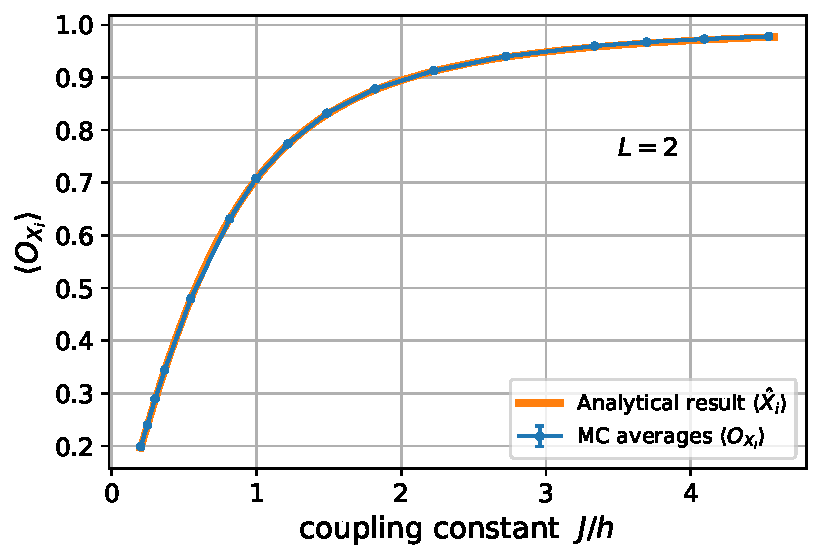
\includegraphics[width=\textwidth]{images/2_site/O_X.pdf}
        \caption{Monte Carlo average $\expval{O_X}$ as a function of $J/h$.}
        \label{expval_O_X_vs_J/h_2}
    \end{subfigure}
\end{figure}
%%% FIG %%%

%%% FIG %%%
\begin{figure}[!htb]\ContinuedFloat
    \centering
    \begin{subfigure}[b]{0.6\textwidth}  %keep total sum <1 to show in same line
        \centering
        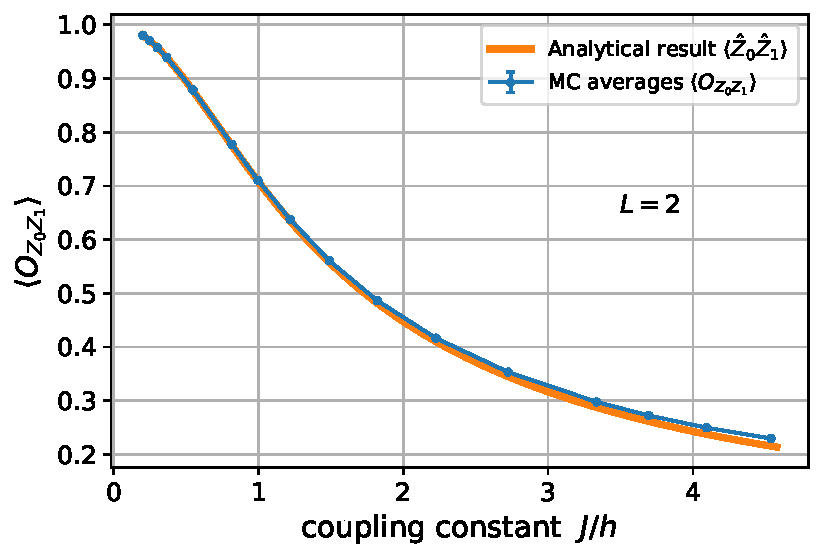
\includegraphics[width=\textwidth]{images/2_site/O_Z0Z1.pdf}
        \caption{Monte Carlo average $\expval{O_{Z_0 Z_1}}$ as a function of $J/h$.}
        \label{expval_O_ZZ_vs_J/h_2}
    \end{subfigure}
    \caption{Comparing analytical results obtained by exactly diagonalizing the quantum Hamiltonian ($d$)  with the numerical results obtained from performing Monte Carlo on the effective classical model $(d+1)$.}
    \label{expval_O_vs_J/h_2}
\end{figure}
\FloatBarrier
As can be seen from Fig. \ref{expval_O_vs_J/h_2}, the Monte Carlo averages of the corresponding classical observables matches with the thermal expectation values of the quantum operators. At higher values of $J/h$, we can see some deviations arising due to the \textit{trotter error} despite the high MC acceptance rate.~\\~\\
Therefore, the algorithm made a first pass on the $2$-site problem, and we expect the algorithm to work for higher values of $N_x$ as well.   

\section{Comparing Monte Carlo with Exact Diagonalization}
Since it is not practical to calculate the analytical expressions for operator thermal expectation values, we perform an Exact Diagonalization (ED) procedure on the quantum Hamiltonian, and calculate the thermal expectation values as 
\begin{equation*}
    \langle \hat{\mathcal{O}} \rangle =  \frac{1}{Z} \Tr(e^{-\beta \hat{H}} \hat{\mathcal{O}}) = \frac{\sum_{i} \mel{E_i}{\hat{\mathcal{O}}}{E_i} \: e^{-\beta E_i}}{\sum_i \braket{E_i}{E_i} e^{-\beta E_i}}
\end{equation*}
where we calculate the trace over the energy eigenbasis. We then compare these quantum thermal expecatation values with the Monte Carlo expectation values of the corresponding classical observables.~\\~\\
For the purposes of our model, $N_x = 13$ is an important lattice size because that is where the subsystem symmetry starts breaking (alignment freezing), and we have to introduce alignment flips to restore ergodicity. Therefore, we compare our ED results for $N_x = 13$ with the MC results, at $\beta =50$, hence doing sufficiently low-temperature studies.

%%% FIG %%%
\begin{figure}[!htb]
    \centering
    \begin{subfigure}[b]{0.6\textwidth}
        \centering
        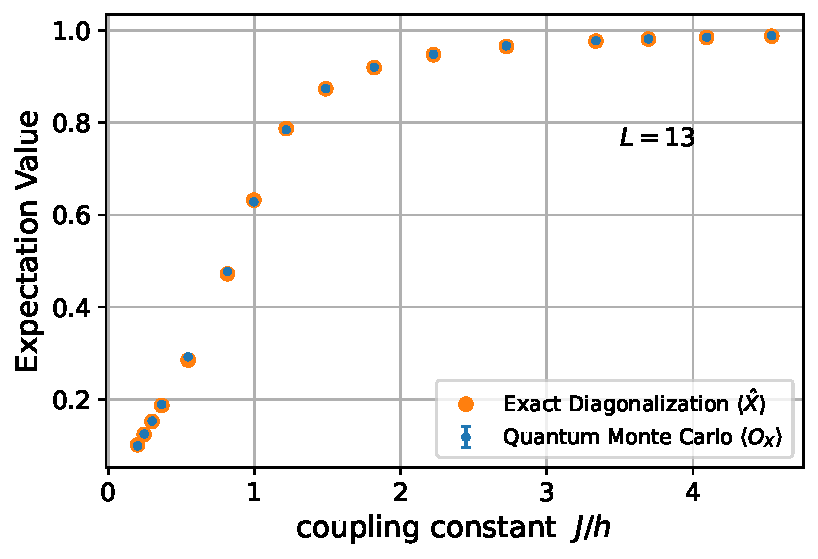
\includegraphics[width=\textwidth]{images/13_site/L=13_X.pdf}
    \end{subfigure}
    \caption{Comparing ED results for $\langle \hat{X} \rangle$ with MC average $\expval{O_X}$ vs. $J/h$.}
    \label{expvalX_ED_vs_MC_13}
\end{figure}
%%% FIG %%%

%%% FIG %%%
\begin{figure}[!htb]
    \centering
    \begin{subfigure}[b]{0.45\textwidth}  %keep total sum <1 to show in same line
        \centering
        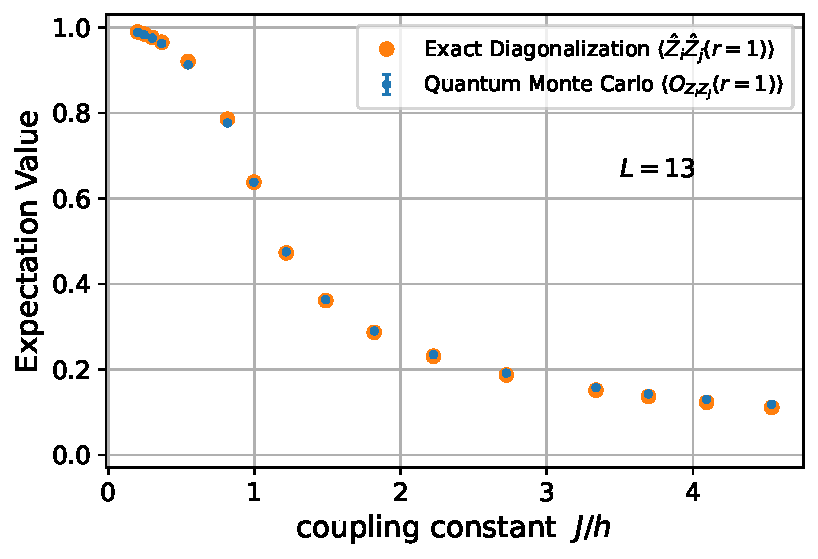
\includegraphics[width=\textwidth]{images/13_site/L=13_ZZ(r=1).pdf}
        \caption{$r \equiv |i-j| = 1$.}
    \end{subfigure}
    \hspace{1em}  %\hfill
    \begin{subfigure}[b]{0.45\textwidth}
        \centering
        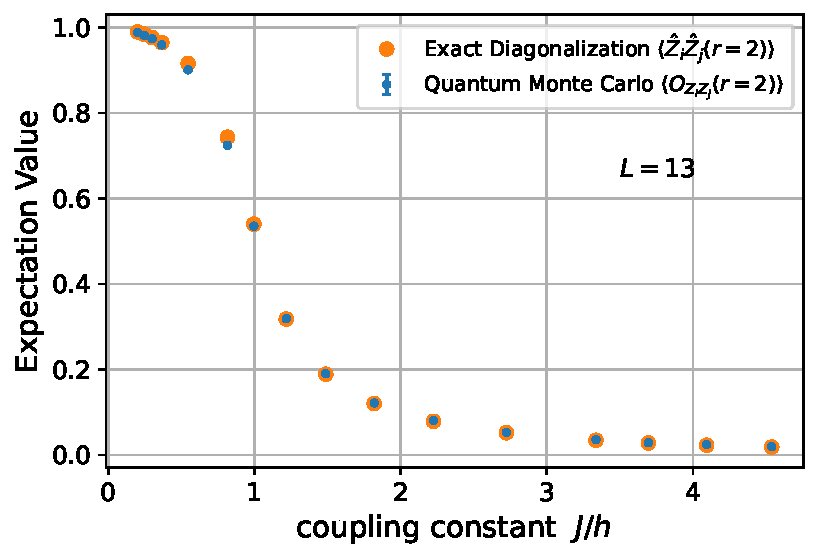
\includegraphics[width=\textwidth]{images/13_site/L=13_ZZ(r=2).pdf}
        \caption{$r \equiv |i-j| = 2$.}
    \end{subfigure}
    \hspace{1em}  %\hfill
    \begin{subfigure}[b]{0.45\textwidth}
        \centering
        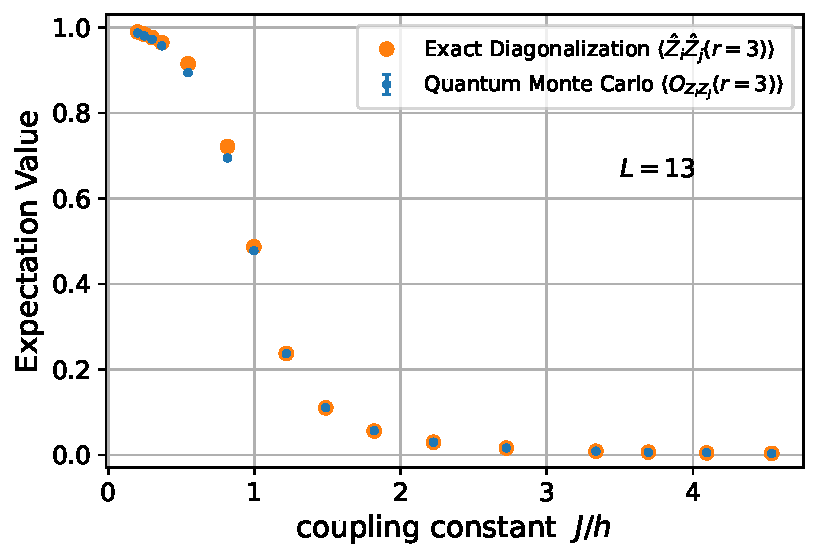
\includegraphics[width=\textwidth]{images/13_site/L=13_ZZ(r=3).pdf}
        \caption{$r \equiv |i-j| = 3$.}
    \end{subfigure}
    \caption{Comparing ED results for $\langle \hat{Z}_i \hat{Z}_j \rangle$ with MC average $\expval{O_{Z_i Z_j}}$ vs. $J/h$.}
    \label{expvalZZ_ED_vs_MC_13}
\end{figure}
\FloatBarrier
\hspace{-1.5em}As can be seen, the results from ED and MC simulations match closely, except for the slight variations in $Z_i Z_j$ expectation values as $|i-j|$ increases, which appear due to periodic boundary effects.~\\~\\
\textcolor{red}{Need to explain exact diagonalization procedure. Add notes.}

\section{Simulations in the limit $\beta \to 0$}
With our machinery set up, we can now attempt to simulate systems in the $\beta < 1$ (or $T>0$) range. However, on staring at the action $S$ of the system for long enough,
\[
    S = -h \Delta\tau \sum_{i=0}^{N_x - 1} \sum_{l=0}^{N_\tau -1} \sigma^{i}_{l} \sigma^{i+1}_{l} - \sum_{l=0}^{N_\tau - 1} \ln \cosh \qty(K N_x A(l)) 
\]
we realize that for a fixed $N_x$ and $N_\tau$, the action primarily depends on two parameters
\[
    Y \equiv h \Delta \tau, \qquad K \equiv -\frac{1}{2} \ln \tanh(J \Delta \tau )
\]  
We can rewrite our coupling constants in terms of the above. Therefore, we realize that \ul{keeping the same values of $Y$, $K$ and $N_\tau$}, we essentially end up solving an entire class of problems (parameterized by the value of $\Delta \tau $) with the following parameters
\begin{align*}
    h = \frac{Y}{\Delta \tau}, \qquad J = \frac{\text{arctanh}(e^{-2K})}{\Delta \tau }, \qquad \beta = N_\tau \Delta \tau. 
\end{align*}
Taking a concrete example, say we perform a MC simulation with $N_\tau = 50$, $h = 0.05$, $K = 2.0$, and $\Delta \tau = 1$. This sets $Y = 0.05$, $K = 2.0$ and $N_\tau = 50$ as fixed values, and the results of this simulation are essentially valid for a class of problems with 
\begin{align*}
    h = \frac{0.05}{\Delta \tau}, \qquad J = \frac{0.18}{\Delta \tau }, \qquad \beta = 50 \Delta \tau. 
\end{align*}  
with any arbitatry $\Delta \tau$. If we choose $\Delta \tau = 0.01$, then our simulation results are valid for the set of parameters $h = 5$, $J = 18$, and $\beta = 0.5$ (or $T = 2$), hence obtaining the results of a high-temperature problem from an equivalent low temperature simulation (with different values of $h$, $J$).

\end{document}